\documentclass[8pt,aspectratio=169]{beamer}
\usetheme{Madrid}
\usecolortheme{default}

\usepackage{amsmath,amssymb,amsthm}
\usepackage{graphicx}
\usepackage{booktabs}
\usepackage{algorithm}
\usepackage{algpseudocode}
\usepackage{tikz}
\usetikzlibrary{arrows.meta,positioning,shapes.geometric}

\title{Deep Generative Models for Private Credit}
\subtitle{Mathematical Foundations and Architecture}
\author{Digital AI Finance}
\date{2026}

\setbeamertemplate{navigation symbols}{}
\setbeamertemplate{footline}[frame number]

\begin{document}

\begin{frame}
\titlepage
\end{frame}

\begin{frame}{Outline}
\tableofcontents
\end{frame}

%------------------------------------------------------------
\section{Introduction}
%------------------------------------------------------------

\begin{frame}{Problem Statement}
\textbf{Challenge}: Model credit risk for private credit portfolios

\vspace{0.5em}
\textbf{Requirements}:
\begin{itemize}
    \item Generate realistic macro scenarios
    \item Capture loan-level heterogeneity
    \item Model temporal dynamics
    \item Enable stress testing
\end{itemize}

\vspace{0.5em}
\textbf{Solution}: Hierarchical deep generative framework
\begin{enumerate}
    \item Macro VAE: Scenario generation
    \item Transition Transformer: Cohort dynamics
    \item Loan Trajectory Model: Individual paths
    \item Portfolio Aggregator: Waterfall mechanics
\end{enumerate}
\end{frame}

\begin{frame}{Hierarchical Framework}
\begin{center}
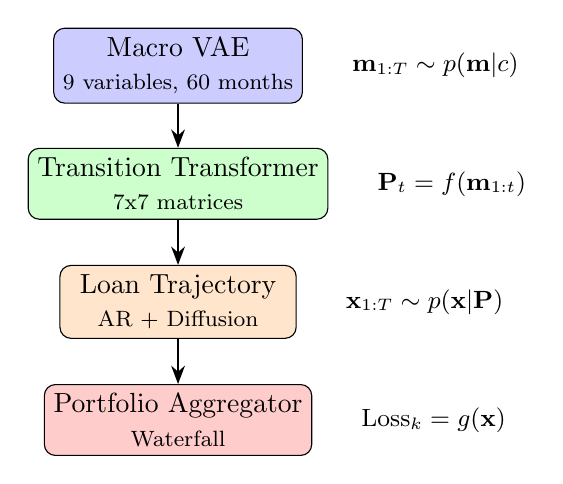
\begin{tikzpicture}[
    box/.style={rectangle, draw, rounded corners, minimum width=3cm, minimum height=0.8cm, align=center},
    arrow/.style={-{Stealth}, thick}
]
\node[box, fill=blue!20] (macro) at (0,3) {Macro VAE\\{\footnotesize 9 variables, 60 months}};
\node[box, fill=green!20] (trans) at (0,1.5) {Transition Transformer\\{\footnotesize 7x7 matrices}};
\node[box, fill=orange!20] (loan) at (0,0) {Loan Trajectory\\{\footnotesize AR + Diffusion}};
\node[box, fill=red!20] (port) at (0,-1.5) {Portfolio Aggregator\\{\footnotesize Waterfall}};

\draw[arrow] (macro) -- (trans);
\draw[arrow] (trans) -- (loan);
\draw[arrow] (loan) -- (port);

\node[right=0.5cm of macro, align=left, font=\small] {$\mathbf{m}_{1:T} \sim p(\mathbf{m}|c)$};
\node[right=0.5cm of trans, align=left, font=\small] {$\mathbf{P}_t = f(\mathbf{m}_{1:t})$};
\node[right=0.5cm of loan, align=left, font=\small] {$\mathbf{x}_{1:T} \sim p(\mathbf{x}|\mathbf{P})$};
\node[right=0.5cm of port, align=left, font=\small] {$\text{Loss}_k = g(\mathbf{x})$};
\end{tikzpicture}
\end{center}
\end{frame}

%------------------------------------------------------------
\section{Conditional VAE Theory}
%------------------------------------------------------------

\begin{frame}{Variational Autoencoder Objective}
\textbf{Goal}: Learn $p_\theta(\mathbf{x}|c)$ for macro time series $\mathbf{x}$ given scenario $c$

\vspace{0.5em}
\textbf{Evidence Lower Bound (ELBO)}:
\begin{equation}
\log p_\theta(\mathbf{x}|c) \geq \underbrace{\mathbb{E}_{q_\phi}[\log p_\theta(\mathbf{x}|\mathbf{z},c)]}_{\text{Reconstruction}} - \underbrace{D_{KL}(q_\phi(\mathbf{z}|\mathbf{x},c) \| p(\mathbf{z}|c))}_{\text{Regularization}}
\end{equation}

\vspace{0.5em}
\textbf{Key components}:
\begin{itemize}
    \item $q_\phi(\mathbf{z}|\mathbf{x},c)$: Encoder (recognition model)
    \item $p_\theta(\mathbf{x}|\mathbf{z},c)$: Decoder (generative model)
    \item $p(\mathbf{z}|c)$: Prior (scenario-dependent)
\end{itemize}
\end{frame}

\begin{frame}{Reparameterization Trick}
\textbf{Problem}: Cannot backpropagate through sampling

\vspace{0.5em}
\textbf{Solution}: Reparameterize the random variable
\begin{equation}
\mathbf{z} = \boldsymbol{\mu}_\phi(\mathbf{x},c) + \boldsymbol{\sigma}_\phi(\mathbf{x},c) \odot \boldsymbol{\epsilon}, \quad \boldsymbol{\epsilon} \sim \mathcal{N}(\mathbf{0}, \mathbf{I})
\end{equation}

\vspace{0.5em}
\textbf{Gradient computation}:
\begin{equation}
\nabla_\phi \mathbb{E}_{q_\phi}[f(\mathbf{z})] = \mathbb{E}_{\boldsymbol{\epsilon}}\left[\nabla_\phi f(\boldsymbol{\mu}_\phi + \boldsymbol{\sigma}_\phi \odot \boldsymbol{\epsilon})\right]
\end{equation}

\vspace{0.5em}
Enables end-to-end training via gradient descent.
\end{frame}

\begin{frame}{KL Divergence Closed Form}
For Gaussian distributions with diagonal covariance:

\begin{equation}
D_{KL}\big(\mathcal{N}(\boldsymbol{\mu}, \text{diag}(\boldsymbol{\sigma}^2)) \| \mathcal{N}(\mathbf{0}, \mathbf{I})\big) = \frac{1}{2}\sum_{j=1}^d \left(\sigma_j^2 + \mu_j^2 - 1 - \log\sigma_j^2\right)
\end{equation}

\vspace{0.5em}
\textbf{Interpretation}:
\begin{itemize}
    \item Penalizes deviation from standard normal
    \item Encourages $\mu_j \approx 0$ and $\sigma_j \approx 1$
    \item Balances with reconstruction term
\end{itemize}
\end{frame}

\begin{frame}{KL Annealing}
\textbf{Problem}: Posterior collapse (encoder ignores input)

\vspace{0.5em}
\textbf{Solution}: Cyclical annealing schedule
\begin{equation}
\mathcal{L}_\beta = \mathbb{E}_{q_\phi}[\log p_\theta(\mathbf{x}|\mathbf{z},c)] - \beta_t \cdot D_{KL}(q_\phi \| p)
\end{equation}

\vspace{0.5em}
\textbf{Schedule}:
\begin{equation}
\beta_t = \min\left(1, \frac{t \mod C}{r \cdot C}\right)
\end{equation}

\begin{itemize}
    \item $C$: Cycle length (e.g., 10 epochs)
    \item $r$: Warmup fraction (e.g., 0.5)
    \item Start with $\beta=0$ (pure reconstruction)
    \item Gradually increase to $\beta=1$
\end{itemize}
\end{frame}

%------------------------------------------------------------
\section{Markov Chain Transitions}
%------------------------------------------------------------

\begin{frame}{Credit State Space}
\textbf{7-state Markov chain}:

\begin{table}
\centering
\begin{tabular}{clcc}
\toprule
State & Name & Type & Typical Rate \\
\midrule
0 & Performing & Transient & Base \\
1 & 30 DPD & Transient & 3\% \\
2 & 60 DPD & Transient & 1\% \\
3 & 90+ DPD & Transient & 0.5\% \\
4 & Default & Absorbing & 0.2\% \\
5 & Prepaid & Absorbing & 1.5\% \\
6 & Matured & Absorbing & -- \\
\bottomrule
\end{tabular}
\end{table}

\vspace{0.5em}
Transition matrix $\mathbf{P} \in [0,1]^{7 \times 7}$ with row sums = 1.
\end{frame}

\begin{frame}{Absorbing State Theory}
\textbf{Canonical form}:
\begin{equation}
\mathbf{P} = \begin{pmatrix} \mathbf{Q} & \mathbf{R} \\ \mathbf{0} & \mathbf{I} \end{pmatrix}
\end{equation}

\vspace{0.5em}
\textbf{Fundamental matrix}:
\begin{equation}
\mathbf{N} = (\mathbf{I} - \mathbf{Q})^{-1} = \sum_{k=0}^{\infty} \mathbf{Q}^k
\end{equation}

$N_{ij}$ = expected time in state $j$ starting from $i$ before absorption.

\vspace{0.5em}
\textbf{Absorption probabilities}:
\begin{equation}
\mathbf{B} = \mathbf{N}\mathbf{R}
\end{equation}

$B_{i,\text{default}}$ = probability of default starting from state $i$.
\end{frame}

\begin{frame}{Neural Network Parameterization}
\textbf{Softmax constraint}: Ensure valid probabilities
\begin{equation}
P_{ij} = \frac{\exp(f_{ij})}{\sum_{k=0}^{6} \exp(f_{ik})}
\end{equation}

where $f_{ij}$ are unconstrained logits from the network.

\vspace{0.5em}
\textbf{Absorbing state masking}:
\begin{equation}
f_{ij} = \begin{cases}
+\infty & i = j \in \{4,5,6\} \\
-\infty & i \neq j, i \in \{4,5,6\}
\end{cases}
\end{equation}

Guarantees absorbing states remain absorbing.
\end{frame}

\begin{frame}{Cross-Attention Mechanism}
\textbf{Macro-conditional transitions}:
\begin{equation}
\mathbf{h}_t = \text{CrossAttn}(\mathbf{s}_t, \mathbf{m}_{1:T})
\end{equation}

\begin{equation}
= \text{Softmax}\left(\frac{\mathbf{s}_t \mathbf{W}_Q (\mathbf{m}_{1:T}\mathbf{W}_K)^\top}{\sqrt{d_k}}\right) \mathbf{m}_{1:T}\mathbf{W}_V
\end{equation}

\vspace{0.5em}
\textbf{Effect}: Transitions depend on macro environment
\begin{itemize}
    \item High unemployment $\rightarrow$ higher default transitions
    \item Low GDP growth $\rightarrow$ fewer prepayments
    \item Credit spread widening $\rightarrow$ stressed matrices
\end{itemize}
\end{frame}

%------------------------------------------------------------
\section{Diffusion Models}
%------------------------------------------------------------

\begin{frame}{Forward Diffusion Process}
\textbf{Gradually add noise}:
\begin{equation}
q(\mathbf{x}_t | \mathbf{x}_{t-1}) = \mathcal{N}(\mathbf{x}_t; \sqrt{1-\beta_t}\mathbf{x}_{t-1}, \beta_t\mathbf{I})
\end{equation}

\vspace{0.5em}
\textbf{Direct sampling} (closed form):
\begin{equation}
q(\mathbf{x}_t | \mathbf{x}_0) = \mathcal{N}(\mathbf{x}_t; \sqrt{\bar{\alpha}_t}\mathbf{x}_0, (1-\bar{\alpha}_t)\mathbf{I})
\end{equation}

where $\bar{\alpha}_t = \prod_{s=1}^t (1-\beta_s)$.

\vspace{0.5em}
\textbf{Reparameterization}:
\begin{equation}
\mathbf{x}_t = \sqrt{\bar{\alpha}_t}\mathbf{x}_0 + \sqrt{1-\bar{\alpha}_t}\boldsymbol{\epsilon}, \quad \boldsymbol{\epsilon} \sim \mathcal{N}(\mathbf{0}, \mathbf{I})
\end{equation}
\end{frame}

\begin{frame}{Reverse Process}
\textbf{Learn to denoise}:
\begin{equation}
p_\theta(\mathbf{x}_{t-1} | \mathbf{x}_t) = \mathcal{N}(\mathbf{x}_{t-1}; \boldsymbol{\mu}_\theta(\mathbf{x}_t, t), \sigma_t^2\mathbf{I})
\end{equation}

\vspace{0.5em}
\textbf{Mean prediction} (noise parameterization):
\begin{equation}
\boldsymbol{\mu}_\theta(\mathbf{x}_t, t) = \frac{1}{\sqrt{\alpha_t}}\left(\mathbf{x}_t - \frac{\beta_t}{\sqrt{1-\bar{\alpha}_t}}\boldsymbol{\epsilon}_\theta(\mathbf{x}_t, t)\right)
\end{equation}

\vspace{0.5em}
\textbf{Training objective} (simplified):
\begin{equation}
\mathcal{L} = \mathbb{E}_{t, \mathbf{x}_0, \boldsymbol{\epsilon}}\left[\|\boldsymbol{\epsilon} - \boldsymbol{\epsilon}_\theta(\mathbf{x}_t, t)\|^2\right]
\end{equation}
\end{frame}

\begin{frame}{DDPM Sampling Algorithm}
\begin{algorithm}[H]
\caption{DDPM Sampling}
\begin{algorithmic}[1]
\State $\mathbf{x}_T \sim \mathcal{N}(\mathbf{0}, \mathbf{I})$
\For{$t = T, T-1, \ldots, 1$}
    \State $\mathbf{z} \sim \mathcal{N}(\mathbf{0}, \mathbf{I})$ if $t > 1$, else $\mathbf{z} = \mathbf{0}$
    \State $\mathbf{x}_{t-1} = \frac{1}{\sqrt{\alpha_t}}\left(\mathbf{x}_t - \frac{\beta_t}{\sqrt{1-\bar{\alpha}_t}}\boldsymbol{\epsilon}_\theta(\mathbf{x}_t, t)\right) + \sigma_t \mathbf{z}$
\EndFor
\State \Return $\mathbf{x}_0$
\end{algorithmic}
\end{algorithm}

\vspace{0.5em}
\textbf{Variance choices}:
\begin{itemize}
    \item $\sigma_t^2 = \beta_t$: Standard
    \item $\sigma_t^2 = \tilde{\beta}_t = \frac{1-\bar{\alpha}_{t-1}}{1-\bar{\alpha}_t}\beta_t$: Posterior variance
\end{itemize}
\end{frame}

%------------------------------------------------------------
\section{Waterfall Mechanics}
%------------------------------------------------------------

\begin{frame}{CLO Tranche Structure}
\textbf{Loss allocation formula}:
\begin{equation}
\ell_k(L) = \min\left(\max\left(\frac{L - A_k}{D_k - A_k}, 0\right), 1\right)
\end{equation}

where $A_k$ = attachment, $D_k$ = detachment.

\vspace{0.5em}
\begin{table}
\centering
\begin{tabular}{lccc}
\toprule
Tranche & Attachment & Detachment & Spread \\
\midrule
AAA & 30\% & 100\% & L+120 \\
AA & 22\% & 30\% & L+180 \\
A & 16\% & 22\% & L+250 \\
BBB & 10\% & 16\% & L+350 \\
BB & 5\% & 10\% & L+600 \\
Equity & 0\% & 5\% & Residual \\
\bottomrule
\end{tabular}
\end{table}
\end{frame}

\begin{frame}{Differentiable Approximation}
\textbf{Problem}: $\min$/$\max$ not differentiable

\vspace{0.5em}
\textbf{Solution}: Soft gating functions
\begin{equation}
\ell_k^{\text{soft}}(L; \tau) = \sigma\left(\frac{L - A_k}{\tau}\right) \cdot \left(1 - \sigma\left(\frac{L - D_k}{\tau}\right)\right) \cdot \frac{L - A_k}{D_k - A_k}
\end{equation}

where $\sigma(x) = 1/(1+e^{-x})$ and $\tau$ controls sharpness.

\vspace{0.5em}
\textbf{Temperature annealing}:
\begin{itemize}
    \item Start with $\tau = 0.1$ (smooth gradients)
    \item Anneal to $\tau = 0.001$ (accurate allocation)
    \item Enables end-to-end training
\end{itemize}
\end{frame}

%------------------------------------------------------------
\section{Risk Metrics}
%------------------------------------------------------------

\begin{frame}{Value at Risk (VaR)}
\textbf{Definition}: $\alpha$-quantile of loss distribution
\begin{equation}
\text{VaR}_\alpha(L) = F_L^{-1}(\alpha) = \inf\{x : \mathbb{P}(L \leq x) \geq \alpha\}
\end{equation}

\vspace{0.5em}
\textbf{Parametric} (Normal):
\begin{equation}
\text{VaR}_\alpha = \mu + \sigma \Phi^{-1}(\alpha)
\end{equation}

\vspace{0.5em}
\textbf{Limitation}: Not subadditive
\begin{equation}
\text{VaR}_\alpha(L_1 + L_2) \not\leq \text{VaR}_\alpha(L_1) + \text{VaR}_\alpha(L_2)
\end{equation}

Diversification may appear to increase risk!
\end{frame}

\begin{frame}{Conditional VaR (CVaR)}
\textbf{Definition}: Expected loss beyond VaR
\begin{equation}
\text{CVaR}_\alpha(L) = \mathbb{E}[L | L \geq \text{VaR}_\alpha(L)] = \frac{1}{1-\alpha}\int_\alpha^1 \text{VaR}_u(L)\, du
\end{equation}

\vspace{0.5em}
\textbf{Parametric} (Normal):
\begin{equation}
\text{CVaR}_\alpha = \mu + \sigma \frac{\phi(\Phi^{-1}(\alpha))}{1-\alpha}
\end{equation}

\vspace{0.5em}
\textbf{Key property}: Coherent risk measure
\begin{itemize}
    \item Subadditive: $\text{CVaR}(L_1 + L_2) \leq \text{CVaR}(L_1) + \text{CVaR}(L_2)$
    \item Captures tail risk better than VaR
\end{itemize}
\end{frame}

%------------------------------------------------------------
\section{Training Procedure}
%------------------------------------------------------------

\begin{frame}{Multi-Stage Training}
\textbf{Stage 1}: Train Macro VAE
\begin{itemize}
    \item Input: Historical macro data by scenario
    \item Loss: ELBO with KL annealing
    \item Epochs: 100-200
\end{itemize}

\vspace{0.5em}
\textbf{Stage 2}: Train Transition Transformer
\begin{itemize}
    \item Input: Macro paths + cohort transitions
    \item Loss: Cross-entropy on transition matrices
    \item Epochs: 50-100
\end{itemize}

\vspace{0.5em}
\textbf{Stage 3}: Train Loan Trajectory Model
\begin{itemize}
    \item Input: Individual loan paths
    \item Loss: Diffusion noise prediction + state classification
    \item Epochs: 100-200
\end{itemize}
\end{frame}

\begin{frame}{End-to-End Fine-tuning}
\textbf{Joint optimization}:
\begin{equation}
\mathcal{L}_{\text{total}} = \mathcal{L}_{\text{VAE}} + \lambda_1 \mathcal{L}_{\text{trans}} + \lambda_2 \mathcal{L}_{\text{traj}} + \lambda_3 \mathcal{L}_{\text{waterfall}}
\end{equation}

\vspace{0.5em}
\textbf{Differentiable waterfall} enables:
\begin{itemize}
    \item Backprop through entire pipeline
    \item Optimize for downstream risk metrics
    \item Scenario-specific fine-tuning
\end{itemize}

\vspace{0.5em}
\textbf{Practical tips}:
\begin{itemize}
    \item Freeze early stages initially
    \item Gradually unfreeze for fine-tuning
    \item Use smaller learning rate for frozen layers
\end{itemize}
\end{frame}

%------------------------------------------------------------
\section{Summary}
%------------------------------------------------------------

\begin{frame}{Key Takeaways}
\begin{enumerate}
    \item \textbf{Conditional VAE}: Generate macro scenarios with ELBO objective
    \item \textbf{Markov Chains}: Model credit states with absorbing state theory
    \item \textbf{Diffusion}: Generate continuous outputs with denoising
    \item \textbf{Waterfall}: Allocate losses to tranches differentiably
    \item \textbf{Risk Metrics}: CVaR preferred over VaR for coherence
\end{enumerate}

\vspace{1em}
\textbf{Framework advantages}:
\begin{itemize}
    \item Hierarchical structure captures dependencies
    \item End-to-end differentiable
    \item Supports stress testing and scenario analysis
\end{itemize}
\end{frame}

\begin{frame}{References}
\begin{thebibliography}{9}
\bibitem{kingma2014} Kingma, D.P. \& Welling, M. (2014). Auto-encoding variational Bayes. \textit{ICLR}.
\bibitem{ho2020} Ho, J., et al. (2020). Denoising diffusion probabilistic models. \textit{NeurIPS}.
\bibitem{vaswani2017} Vaswani, A., et al. (2017). Attention is all you need. \textit{NeurIPS}.
\bibitem{artzner1999} Artzner, P., et al. (1999). Coherent measures of risk. \textit{Mathematical Finance}.
\bibitem{jarrow1997} Jarrow, R., et al. (1997). A Markov model for credit risk spreads. \textit{RFS}.
\end{thebibliography}
\end{frame}

\end{document}
